%\documentclass[a4paper,12pt]{book}
%\usepackage{fixltx2e}
%\usepackage{graphicx}	
%\begin{document}
\newpage

\chapter{Background Study and Related Works}
\paragraph{}
In this chapter we describe some related work and provide some background stuffs that are  pertinent to the remainder of this paper.
\section{Data Mining}
What is data mining and frequent pattern mining we have discussed in Chapter 1. Now we discussed related approaches for data mining and frequent pattern mining. There are two common approaches in determining frequent item set. First one is a well known algorithm called Apriori. Apriori is a prior knowledge based  algorithm, that is , if any pattern is not frequent then one of its super-pattern will be frequent.It works in a level wise approach. From the given database in each level it's generate frequent sub-patterns and merges them to propagate the candidates for next level. The second approach is pattern growth e.g., FP-growth method. The FP-Growth methods adopts a divide and conquer strategy as follows: compress the database representing frequent items into a frequent-pattern tree, but retain the itemset association information, and then divide such a compressed database into a set of condition databases, each associated with one frequent item, and mined from the tree. There are no need to generate candidate for next level or no need to generate candidate. Now we given a comparative discussion on this two algorithms or methods. Already we know FP-growth algorithm use divide and conquer strategy approach. That's why in this algorithm needs at most two scans of the database, while the number of database scans for the Apriori algorithm increases with the dimension of the candidate itemsets(Because this approach generate frequent sub-pattern and merges them to generate candidates for next level ). For this reason the performance of FP-growth algorithm is not influenced by the support factor while the performance of the Apriori algorithm decreases with the support factor. Thus prior knowledge based or candidate generating algorithms behave well only for small databases with a large support factor(at least 30\% ).

\section{Uncertain Data Mining}
Data uncertainty is an inherent property in various applications due to reasons such as outdated sources or imprecise measurement. In the age of Big data, uncertainty is one of the defining characteristics of data. Data is constantly growing in volume, variety, velocity and uncertainty. In a large range of applications domains uncertain data is found in abundance.  Today on the web, in sensor networks, within enterprises both in their structured and unstructured sources,in analysis of meteorological trends, of medical behavior of living organisms data are the example of uncertain data. Customer name of a super shop is an real life example of uncertain data.

\begin{figure}[h!]
  \centering
    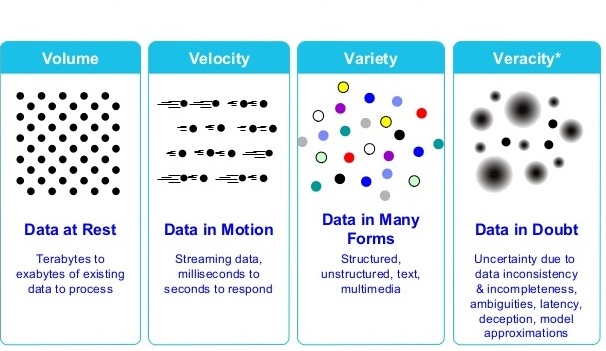
\includegraphics[width=1\textwidth]{images/ra_1}
    \caption{A picture of uncertain data source.}
\end{figure}
In real life we are faced with time series data and features the occurrence of temporal patterns composed of regularity repeating sequences of events, where cyclic activities play a key role.
\begin{figure}
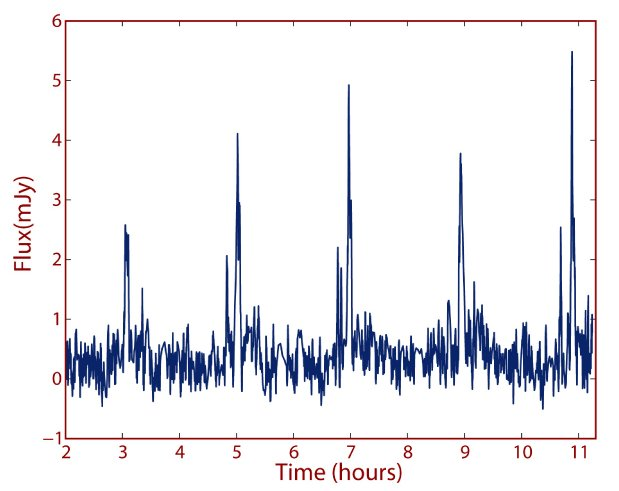
\includegraphics[width=1\textwidth]{images/ra_2}
\caption{A periodic patterns of specific physical medium}
\label{fig:Periodic time series}
\end{figure}
\paragraph{}
An example of periodic time series is given in Figure ~\ref{fig:Periodic time series}, showing the Flux is the presence of a force field in a specified physical medium, or the flow of energy through a surface repetitively occurs. Though consecutive Flux patterns show similar characteristics, they are not equal. It is possible to observe changes in the shape of consecutive periodic patterns that are of significant importance.
\paragraph{}
In the medical domain, physical activity becomes more and more important in the modern society. Nowadays, cardiovascular diseases cover a significant part of a annually occurring affections, which is due to the reduced amount of activity in the daily life. This leads to the research direction of uncertain or probabilistic data. Here, the basic question arises which of these observation in most likely to represent this object. Materialization this likelihood, the observations are associated with probability values; this creates existential dependencies among the observations, as the existence of an observation affects the existence of the other observations of the same object.
\paragraph{}
In the age of big data uncertain data is a common phenomenon.Coping with data uncertainty initiates a need for developing suitable data models and techniques for mining uncertain data. Commonly used models which are used for uncertain data mining are given beneath.
\subsection{Modeling of Uncertain Data}

\begin{figure}[h!]
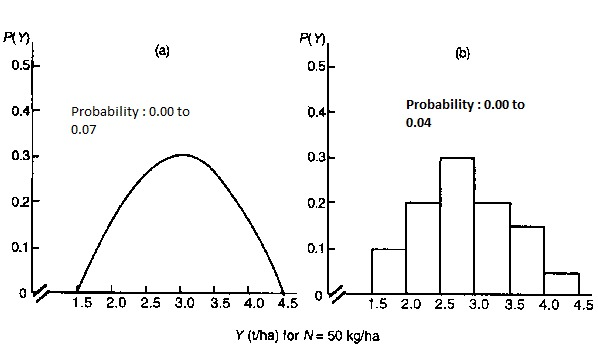
\includegraphics[width=1\textwidth]{images/ra_3}
\caption{Variants of attribute uncertainty}
\label{fig:Uncertainty modeling}
\end{figure}
\subsubsection{Categorization}
There are three main models of uncertain data in databases. In attribute uncertainty, each uncertain attribute in a tuple is subject to its own independent probability distribution. For example, if readings are taken of temperature and wind speed, each would be described by its own probability distribution, as knowing the reading for one measurement would not provide any information about the other.
\paragraph{}
In correlated uncertainty, multiple attributes may be described by a joint probability distribution. For example, if readings are taken of the position of an object, and the x- and y-coordinates stored, the probability of different values may depend on the distance from the recorded coordinates. As distance depends on both coordinates, it may be appropriate to use a joint distribution for these coordinates, as they are not independent.
\paragraph{}
In tuple uncertainty, all the attributes of a tuple are subject to a joint probability distribution. This covers the case of correlated uncertainty, but also includes the case where there is a probability of a tuple not belonging in the relevant relation, which is indicated by all the probabilities not summing to one. For example, assume we have the following tuple from a probabilistic database:
\paragraph{}
$(a, 0.4) | (b, 0.5)$
\paragraph{}
Then, the tuple has 10\% chance of not existing in the database.



\section{Stream Data Mining}
In large application systems or in the age of big data there always needs mining data from continuous or rapid data records. Data Stream Mining is the process of extracting knowledge structures from such kind of data source.A data stream is an ordered sequence of instances that in many applications of data stream mining can be read only once or a small number of times using limited computing and storage capabilities. Example of data source where stream mining is very essential the analysis of meteorological trends, of medical behavior of living organisms, or of recorded physical activity is built on temporally dependent observations or multi observation data, computer network traffic, phone conversations, ATM transactions, web searches, and sensor data.

\paragraph{}
In many data stream mining applications, the goal is to predict the class or value of new instances in the data stream given some knowledge about the class membership or values of previous instances in the data. Data stream mining can be considered a sub-field of data mining stream.
\section{Existing Approaches}
Many algorithms has been developed to mine frequent itemsets from uncertain databases like U-Apriori, UF-growth, UFP-growth, UH-Mine, CUF-growth, CUF-growth, PUF-growth etc.
\subsection{APriori}
Apriori is one of the common algorithm for data mining. It works in a level wise approach based on a prior knowledge. In each level Apriori algorithm generates frequent sub-patterns from the given database and merges them to generate the candidates for next level. That's why this kinds of algorithms called candidates generating algorithm.  Apriori is designed to operate on databases containing transactions (for example, collections of items bought by customers, or details of a website frequentation). Generating frequent sub-patterns it can use large itemset property. The sub-patterns are easily parallelized and it's easy to implement. For those reasons from it's proposed time Apriori is of the frequent used algorithm for data mining.
\paragraph{}
But, some of it's draw back many other algorithms took place over it. The draw back are given below.
\begin{itemize}
 \item Here, number of database scan increases with the dimension of the candidate itemset.
  \item Need transaction databases in memory resident for assumed performance.
\end{itemize}


\subsection{FP growth}
Description
\subsection{U-Priori}
U-Apriori is a  modification of Apriori algorithm which is proposed to handle uncertain data. We already know in Apriori algorithm support count play an important role. Number of databases scan and candidate for next level depends on support count. The modification of Apriori in U-Apriori in support count. Specially, instead of incrementing the support counts of candidate patterns by their actual support, U-Apriori increments the support counts of candidate patterns by their given support count in Apriori. Though U-Apriori come over Apriori to solve support count problem of Apriori but U-Apriori suffers from the following problems:
\begin{itemize}
 \item U-Apriori is a modification of the Apriori algorithm, performance of U-Apriori algorithm for large scale of data because it follows level wise sub-patterns generation and merge to generate candidate for next level. That's why number of databases scan increase with the dimension of itemset.
  \item If the existential probabilities of most items within a pattern I are small, increments for each transaction can be insignificantly small. Consequently, many candidates would not be recognized as infrequent until most transaction were processed.
\end{itemize}
  
\subsection{UF-growth}
Observing outperforms of FP-growth over Apriori UF-growth was proposed for mining uncertain data. We know key to success of FP-growth over Apriori is FP-tree, which is a compact tree structure capturing frequent items within transactions in the databases of precise data. By extracting appropriate tree paths to construct subsequent FP-trees, frequent itemset can be mined. Each tree path represents a transaction. Each node in a tree path captures(i) an item x and (ii) its actual support(i.e, occurrence count of x in that tree path). Tree paths (from the root) are merged if they share the same items(i.e., the captured transaction share the same prefix items). Due to this path sharing, the FP-tree is usually compact. However, when dealing with uncertain data, the situation is different (because each item is associated with an existential probability value). The expected support of any itemset X is the sum of products of existential probability of items within X. Hence, UF-growth uses a UF-tree to capture frequent items within transactions of uncertain data. Each node in an UF-tree captures (i) an item x, (ii) its existential probability value, and (iii) the occurrence count of x in that tree path. By doing so, UF-growth finds all and only those frequent itemsets by computing the expected support of an itemset X (as the sum of products of the captured existential probability values). Tree paths are merged if they share the same items and existential probability values. Consequently, UF-trees may not be as compact as FP-trees.

\subsection{UFP-growth}
To reduce the tree size, UFP-growth groups similar nodes (i.e., nodes with the same x but similar existential probability values) into a cluster. Each cluster of the item x captures (i) the maximum existential probability value of all nodes within the cluster and (ii) the number of existential probability values in each cluster. Depending on the clustering parameter, the resulting tree namely, UFP-tree may be as large as the UF-tree (i.e., no reduction in tree size). On the other hand, if the UFP-tree  is smaller than the UF-tree, then UFP-growth may return approximate results (e.g., with false positives or infrequent itemsets).
\subsection{CUF-growth*}
Description
\subsection{PUF-growth}
To reduce the size of the UF-tree and UFP-tree, the prefix-capped uncertain frequent pattern tree (PUF-tree  structure was proposed, in which important infor- mation about uncertain data is captured so that frequent patterns can be mined from the tree. The PUF-tree  is constructed by considering an upper bound of existential probability value for each item when generating a k-itemset (where k $>$ 1). This upper bound of an item x\textsubscript{r} in a transaction t\textsubscript{j} is called the (prefixed) item cap of x\textsubscript{r} in tj. Thus PUF-tree was compact.
\subsection{SUF-growth}
In this section we propose another algorithm called SUF-growth. SUF-growth algorithm outperforms over UF-streaming algorithm. It improves over UF-streaming by avoiding the aforementioned potential problems for mining frequent itemset from streams of uncertain data. The advantages of SUF-growth over existing others algorithm are given below:
\begin{itemize}
 \item SUF-growth is an exact algorithm. Its means SUF-growth returns only truly frequent itemset. Where UF-streaming returns both true or false frequent itemset.
  \item Its use only minsup. No need to use preMinsup. There also have any problem of finding an appropriate value of preMinsup.
  \item This algorithm does not need UF-stream structure to store the mined itemsets.
  \item Need transaction databases in memory resident for assumed performance. Instead of this its use "delayed" mode for mining. As a result unnecessary computation could be reduced.
\end{itemize}
\paragraph{}
Considering the advantages of SUF-growth over others algorithm there is question. The is how SUF-growth algorithm find frequent itemsets from streams of uncertain data using a new tree structure called SUP-tree. Now we describe about this. We first construct a SUF-tree, and then extract relevant paths from this SUF-tree (which is a global tree) to recursively form smaller UF-trees for projected databases. Due to the dynamic nature and Property 2 of data streams, expected support of items is continuously affected by the arrival of new batches (and the removal of the contents of older batches). Arranging items in frequency-dependent order in the SUF-tree may lead to swapping—which, in turn, can cause merging and splitting—of tree nodes when the global frequencies of items change. Hence, in the SUF-tree, items are arranged according to some canonical order (e.g., lexicographic order), which can be specified by the user prior to the construction of the SUF-tree or the mining process. Consequently, the SUF-tree can be constructed using only one scan of the streams of uncertain data, and the resulting SUF-tree captures the contents of the streams. Moreover, the SUF-tree preserves the usual tree properties:
\begin{itemize}
 \item  The occurrence count of a node is at least as high as the sum of occurrence counts of its children.
  \item The ordering of items is unaffected by the continuous changes in the expected support values of items.
 
\end{itemize}

\section{Summary}
Here is summary.

%\end{document}